\chapter{Experimentos e Resultados}
\label{chap:resultados}
% ----------------------------------------------------------
Este capítulo vem apresentar os experimentos realizados como forma de
verificação do Processo de Avaliação de Capacidade por Inferência de 
Desempenho proposto no Capítulo~\ref{chap:processo}. Inicialmente é
apresentada a metodologia utilizada para construção dos experimentos, 
com a descrição da Aplicação sob Teste escolhida, como foi implantada e 
como foram realizadas as execuções para coleta de dados de desempenho. Depois
são apresentados os resultados obtidos por cada uma das 9 Heurísticas ao
fazer a Avaliação de Capacidade da Aplicação. Esses resultados são usados 
para uma comparação qualitativa das Heusrísticas entre si e para atestar
a eficiência do Processo de Avaliação de Capacidade proposto e sua técnica 
de Inferência de Desempenho tanto quanto à economia de tempo e custo como  
quanto à precisão de acerto de seuas predições.

\section{Metodologia}
\label{sec:resultados_metodologia}
A fim de validar a eficiência da Inferência de Desempenho no apoio
ao Planejamento de Capacidade, foram realizadas seções de avaliação de
capacidade de uma aplicação implantada em um provedor de nuvem de
infraestrutura como serviço.

A aplicação escolhida foi o WordPress \cite{wordpress}, um motor de construção 
e administração de \emph{blogs}. Sua escolha foi motivada por ser uma aplicação
bem conhecida, de utilização via web, ideal para implantação em ambiente de
nuvem, e com componentes arquiteturais escaláveis. Além disso, o fluxo de 
utilização típico apresenta características bem diversificadas quanto ao uso
de recursos de CPU e memória, rede, sistema de arquivos e banco de dados.

\begin{figure}[hbt]
  \caption{\label{fig:implantacao}Implantação do WordPress na AWS EC2 para Avaliação de Capacidade}
  \begin{center}
    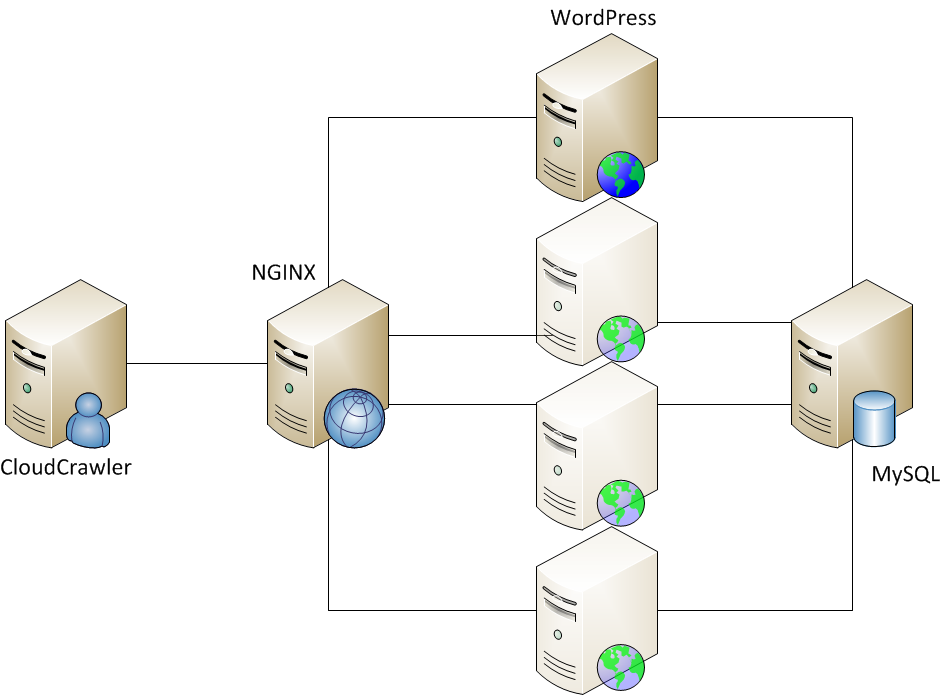
\includegraphics[scale=0.4]{img/ImplantacaoWordPress}
  \end{center}
\end{figure}

O Provedor escolhido foi a Amazon, com seu serviço de infraestrutura AWS EC2
\cite{ec2}, onde o WordPress foi implantado em duas camadas: uma para o banco de 
dados MySQL, e outra para a aplicação, executada pelo servidor Apache HTTPD. Como
balanceador de carga, foi utilizada uma máquina executando o servidor web Nginx. A
Figura~\ref{fig:implantacao} mostra um panorama geral dessa implantação. 

Devido a restrições de custo e tempo, os experimentos foram limitados de forma a variar 
apenas a camada de aplicação, usando de 1 a 4 servidores Apache executando o WordPress. 
Na imagem, essa variação está representada pela suavização de cor das máquinas dessa 
camada, no sentido de que podem não estar presentes em certos cenários.

A execução dos testes foi orquestrada pelo Cloud~Crawler~\cite{cunha2012ambiente},
que automatizou as tarefas de iniciar e parar as todas as instâncias, configurar 
o balanceador de carga de acordo com o número de instâncias testadas na camada de 
aplicação, iniciar e parar a execução dos testes, controlando as Cargas de Trabalho
impostas à Aplicação sob Teste (o WordPress) e coletando os dados de desempenho 
para cada execução. 

De forma a viabilizar uma \emph{baseline} para validação e verificação das 
predições de desempenho inferidas pelo Processo de Avaliação implementado pela 
biblioteca CloudCapacitor, foram efetivamente executados testes de desempenho 
para todas as combinações de Configurações e Cargas de Trabalho. A esse conjunto
de dados reais de execução foi dado o nome de ``oráculo'' e esse procedimento
de teste de todas as possibilidades foi considerado como uma Heurística de ``Força
Bruta''. As 9 Heurísticas propostas no Capítulo~\ref{chap:processo} foram comparadas
entre si e com a Heurística de Força Bruta, que não faz qualquer inferência de
desempenho. O resultado dessas comparações serão analisados nas seções seguintes.

Para compor o Espaço de Implantação do experimento desenvolvido para este trabalho, 
foram escolhidos 7 Tipos de Máquinas Virtuais oferecidos pelo serviço AWS EC2:

\begin{itemize}
  \item m3\_medium 
  \item m3\_large
  \item m3\_xlarge
  \item m3\_2xlarge
  \item c3\_large
  \item c3\_xlarge
  \item c3\_2xlarge
\end{itemize}

Para cada um desses Tipos de Máquinas, foram criadas Configurações com 1, 2, 3 e 4
instâncias, levando a um total de 28 Configurações diferentes no Espaço de Implantação,
divididas em duas Categorias distintas, ``C3'' e ``M3''. As Cargas de Trabalho
para este experimento foram quantificadas em número de usuários fazendo
requisições ao WordPress. Foram criadas 10 Cargas de Trabalho representando
100, 200, 300, 400, 500, 600, 700, 800, 900 e 1000 usuários. Com isso, foram
coletados dados de desempenho para 280 cenários diferentes, ou seja, foram 
testadas as 28 Configurações em cada uma das 10 Cargas de Trabalho especificadas 
para a Avaliação de Capacidade do WordPress na nuvem.

O teste de desempenho consistiu em fazer com que a Aplicação sob Teste WordPress
atendesse à demanda imposta pelo acesso de tantos usuários quanto especificados 
na Carga de Trabalho no período de 1 hora. Cada usuário disparava a seguinte
sequência de requisições:

\begin{enumerate}
  \item Efetuar \emph{logon}
  \item Inserir uma postagem
  \item Visitar uma postagem específica
  \item Alterar uma postagem
  \item Efetuar pesquisa por palavra-chave
  \item Alterar uma postagem
  \item Efetuar \emph{logoff}
\end{enumerate}

A Métrica de Desempenho usada no experimento foi ``Tempo de Resposta Total'', ou 
seja, o tempo total decorrido entre o envio da primeira requisição da sequência 
acima e o momento em que o cliente recebeu a resposta para última requisição da
sequência. Assim, para ser considerada como Candidata, uma Configuração devia 
ser capaz de atender 90\% dos conjuntos de requisições em um tempo total abaixo 
do tempo informado na entrada do parâmetro SLA.

A seguir serão discutidos os resultados obtidos com o Processo de Inferência de 
Desempenho e suas Heurísticas na indicação das Configurações capazes de executar
a Aplicação sob Teste sob vários níveis de demanda. Foram avaliadas a precisão do 
Processo na predição de capacidade e a economia de tempo e custo na execução
dos testes.

\section{Avaliação dos Resultados}
\label{sec:resultados_avaliacao}
A partir da execução do Processo de Inferência de Desempenho implementado pela
biblioteca CloudCapacitor, usada no desenvolvimento do Capacitor Web, foram 
realizadas Avaliações de Capacidade em 280 cenários de implantação do WordPress 
no serviço AWS EC2.

Com base nos resultados desses testes, foram avaliados os seguintes aspectos em
relação ao desempenho do Processo: 

\begin{description}
  \item[Precisão] \hfill \\ Relação entre acertos e erros na predição de 
  capacidade das Configurações    
  \item[Eficiência] \hfill \\ Grau de redução do número de execuções reais e,
  consequentemente, do custo e do tempo total gasto nos testes de desempenho.
\end{description}

\subsection{Precisão}
\label{subsec:resultados_precisao}
A avaliação da Precisão, ou acurácia, das predições realizadas pelo Processo
de Inferência visa a ratificar a expectativa de que, uma vez identificada uma
relação de capacidade entre diferentes Configurações oferecidas por um Provedor
de infraestrutura na nuvem, é possível inferir o desempenho de uma Aplicação
executando em uma Configuração com base no desempenho observado em uma
execução real da Aplicação em uma Configuração distinta.

\begin{figure}[hbt]
  \caption{\label{fig:avaliacao_precisao}Avaliação da Precisão da Inferência de Desempenho}
  \begin{center}
    \includegraphics[scale=0.5]{img/Precision}
  \end{center}
\end{figure}

Assim, este trabalho submeteu o Processo à verificação de sua acurácia ao realizar
predições para o desempenho do WordPress executando em máquinas virtuais do provedor
Amazon Web Services. O cálculo de Precision and Recall~\cite{powers2011evaluation} 
sobre os resultados dos experimentos realizados mostra que o Processo de Inferência 
de Desempenho é capaz de obter índices de precisão muito próximos de 100\%, como 
pode ser observado na Figura~\ref{fig:avaliacao_precisao}. 

A imagem mostra XXXXXXXXXXXXXXXXXXXXXXXXXXXXXXXXXXXXXXXXXXXXXX

Isso significa que, com a correta representação das relações de capacidade entre
as Configurações, o Processo de Inferência de Desempenho proposto neste trabalho
consegue efeticamente predizer, com grande confiança, quais Configurações de um 
Provedor são capazes de executar uma Aplicação sob os níveis de demanda analisados. 

\subsection{Eficiência}
\label{subsec:resultados_eficiencia}
Esta seção apresenta os resultados de eficiência atingidos pelas Heurísticas usadas 
pelo Processo de Inferência de Desempenho sob dois aspectos distintos: o custo 
total da Avaliação e a quantidade de execuções realizadas pelas Heurísticas. Esse 
custo foi calculado somando-se o preço da hora de utilização, conforme a tabela 
de preços do provedor na data realização dos testes, para cada uma das Configurações 
para as quais foram realizadas execuções reais na nuvem. 

\begin{figure}[hbt]
  \caption{\label{fig:eficiencia_custo}Avaliação da Eficiência de Custo das Heurísticas}
  \centering
    \begin{subfigure}[a]{0.7\textwidth}
      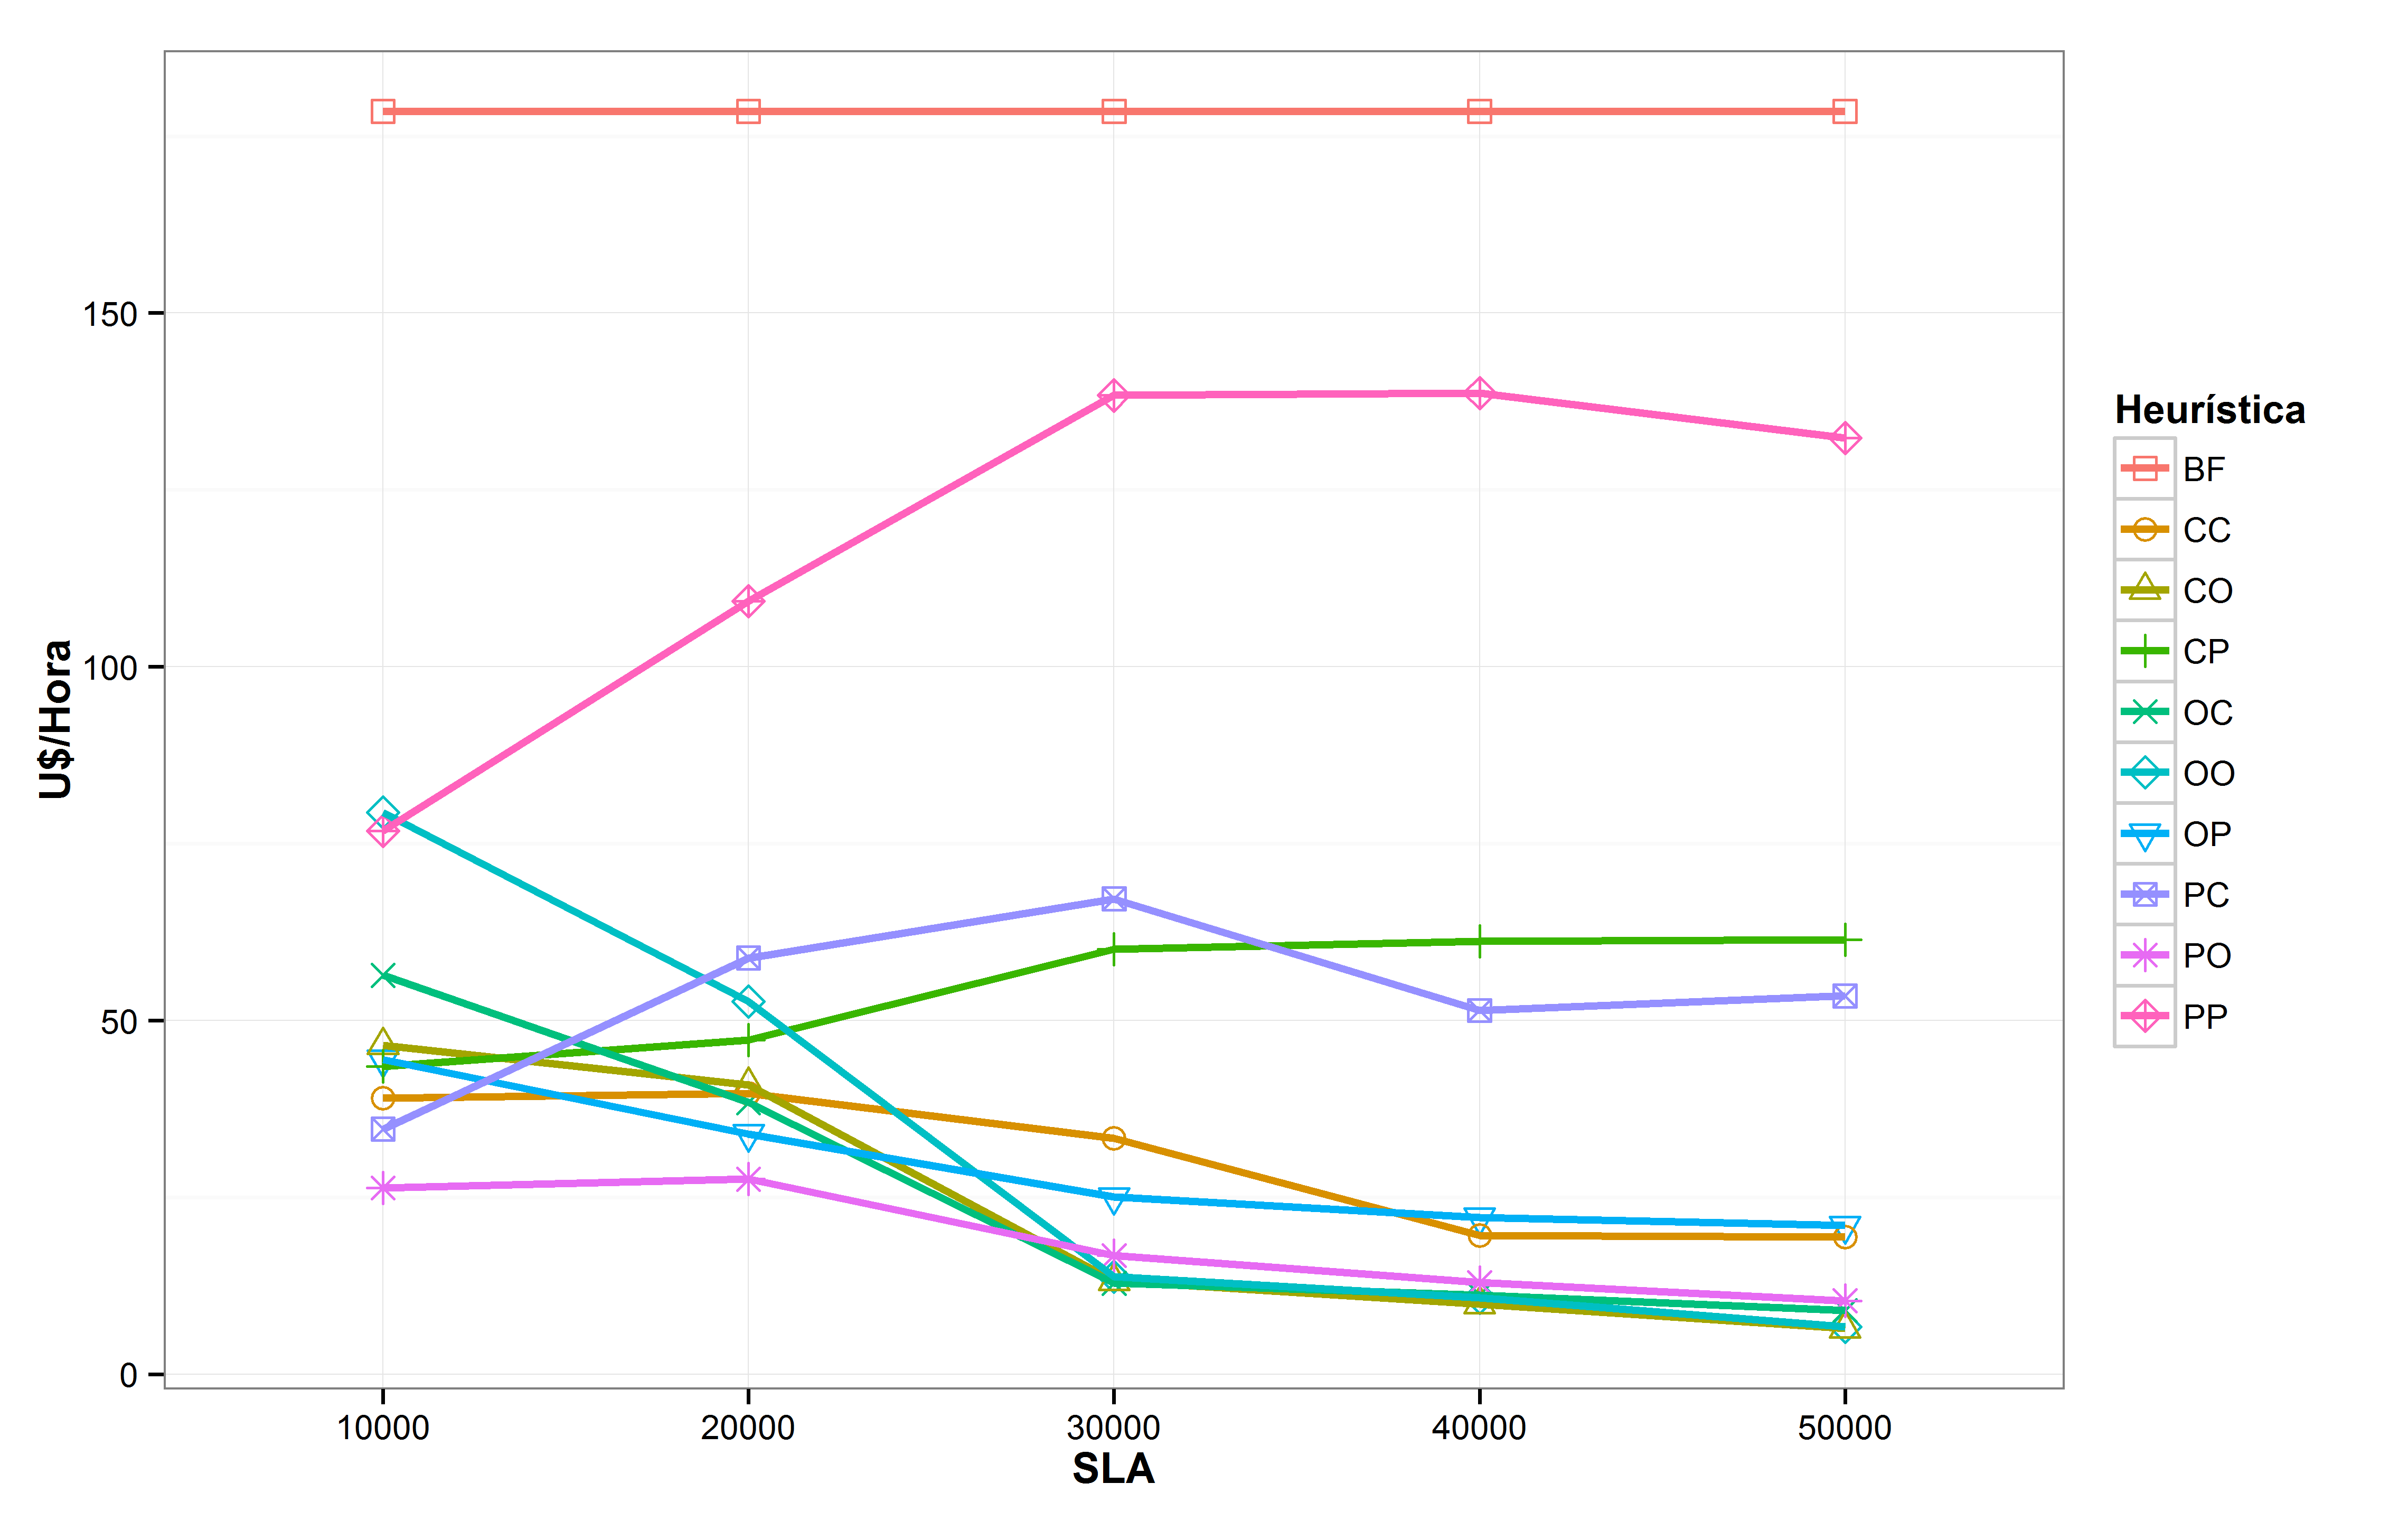
\includegraphics[width=\textwidth]{img/ExecutionCost-Capacity}
      \caption{Grafo por Capacidade}
      \label{fig:eficiencia_custo_capacidade}
    \end{subfigure}
    \begin{subfigure}[b]{0.7\textwidth}
      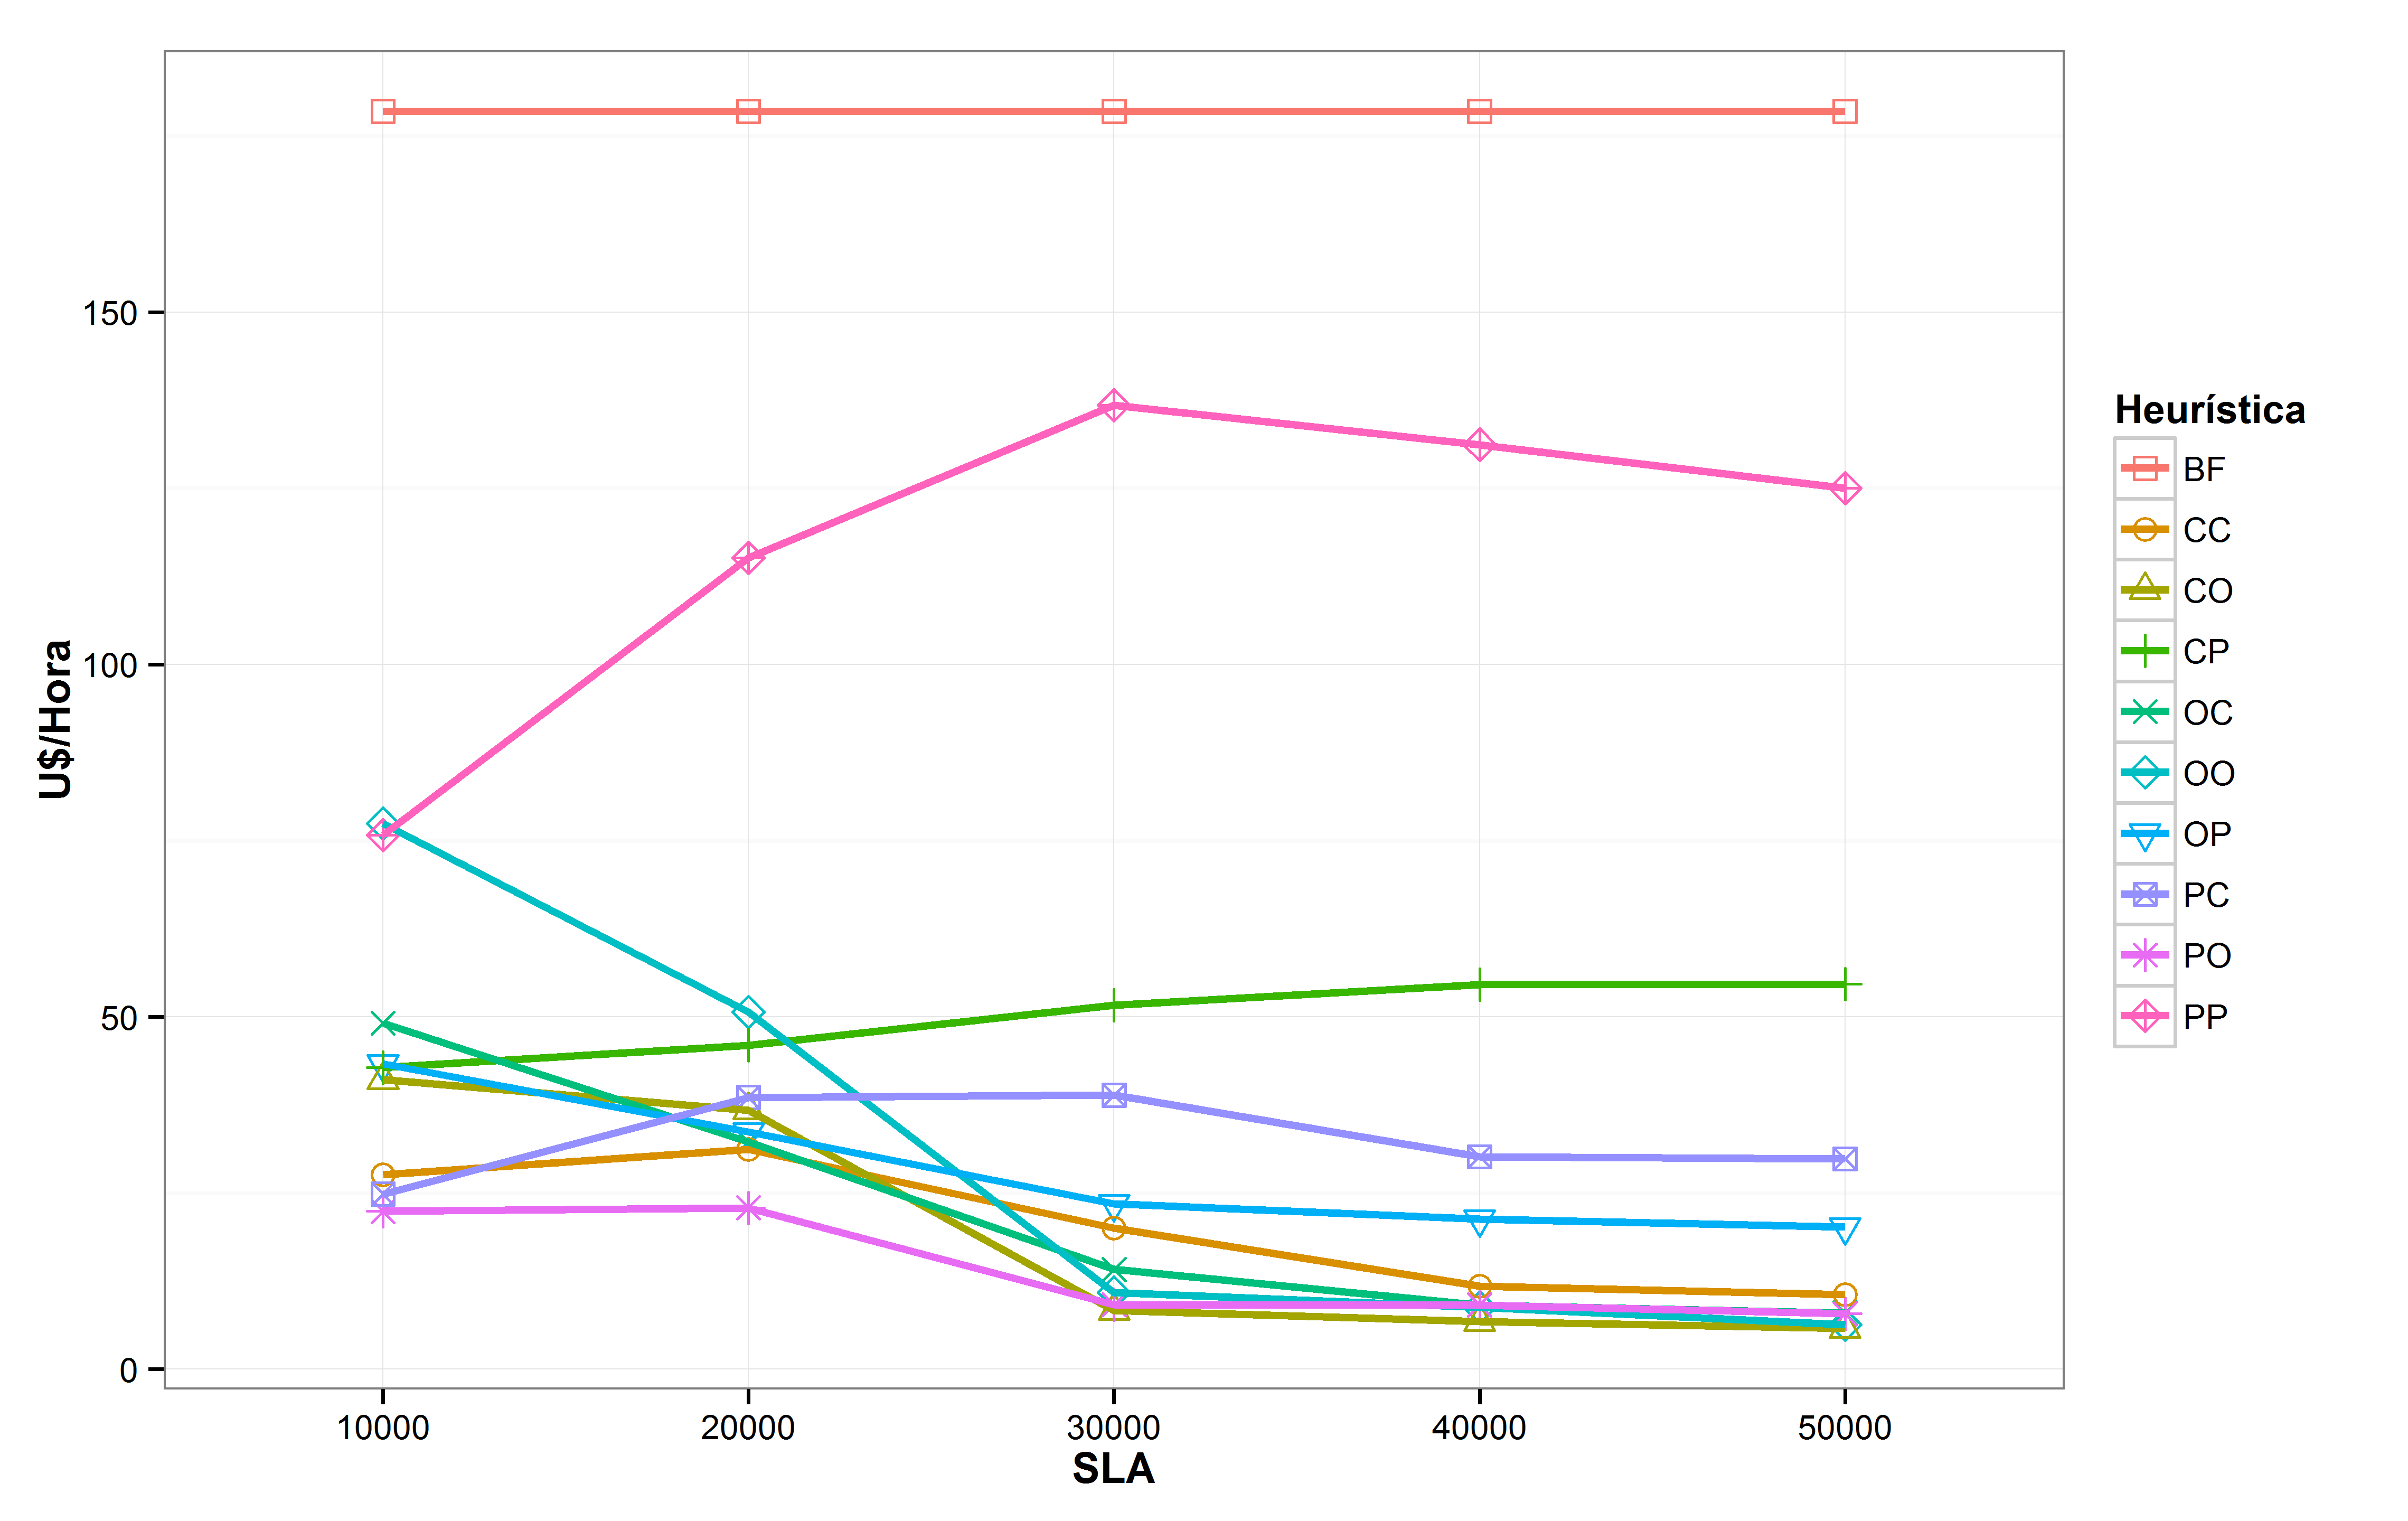
\includegraphics[width=\textwidth]{img/ExecutionCost-Price}
      \caption{Grafo por Preço}
      \label{fig:eficiencia_custo_preco}
    \end{subfigure}
\end{figure}

Para cada aspecto analisado, custo e número de execuções, foram realizadas duas 
baterias iguais de testes, uma utilizando o Espaço de Implantação gerado com base 
nas relações de poder computacional entre as Configurações e outra com o Espaço de 
Implantação baseado nas relações de preço. Essa variação foi feita para que fosse
possível estudar o efeito da regra de formação do Espaço de Implantação sobre o
desempenho geral do Processo de Inferência de Desempenho. Embora haja alguma 
diferença entre os resultados obtidos com ambas as representações, a percepção 
geral da eficiência das Heurísticas não muda.   

A Figura~\ref{fig:eficiencia_custo} mostra os gráficos dos resultados obtidos pelas
9 Heurísticas em termos de custo total dos testes de Avaliação considerando SLAs 
entre 10 e 50 segundos. O primeiro gráfico apresenta os resultados quando os testes
foram executados com a representação do Espaço de Implantação baseado na relação de
capacidade entre as Configurações. O segundo gráfico considera o grafo da relação
de preço das Configurações usado para representar o Espaço de Implantação.

No topo de ambos os gráficos vê-se um linha horizontal que representa a 
\emph{baseline} de comparação, que é o custo total da Heurística de Força Bruta 
(\emph{Brute Force - BF}). Como o custo total para execução da Aplicação em todas
as combinações de Configurações e Cargas de Trabalho é sempre o mesmo, independente
do SLA requerido, a linha do gráfico para essa Heurística sempre é uma linha
horizontal.

A análise das imagens dos gráficos mostra que mesmo a Heurística com o pior 
desempenho no que se refere ao custo total da Avaliação já apresenta uma redução 
em relação à Força Bruta. Por outro lado, as melhores Heurísticas chegam a 
representar uma economia da ordem de 96\% em comparação com o que seria gasto
com a execução de todas as combinações de Configurações e Cargas de Trabalho.

Embora o comportamento das Heurísticas varie em função do SLA, é possível notar
que quando a exigência do SLA é mais moderada o comportamento de todas as Heurísticas
tende a se estabilizar, tornando possível identificar que algumas delas tendem a
ser mais econômicas que as outras. Ainda que não seja possível afirmar uma só 
Heurística como a melhor em todas as situações, pode-se considerar que as Heurísticas
Pessimista~Otimista e Conservadora~Otimista se mostram mais econômicas em geral.
 
\begin{figure}[hbt]
  \caption{\label{fig:eficiencia_execucoes}Avaliação da Eficiência do Número de Execuções das Heurísticas}
  \centering
    \begin{subfigure}[a]{0.7\textwidth}
      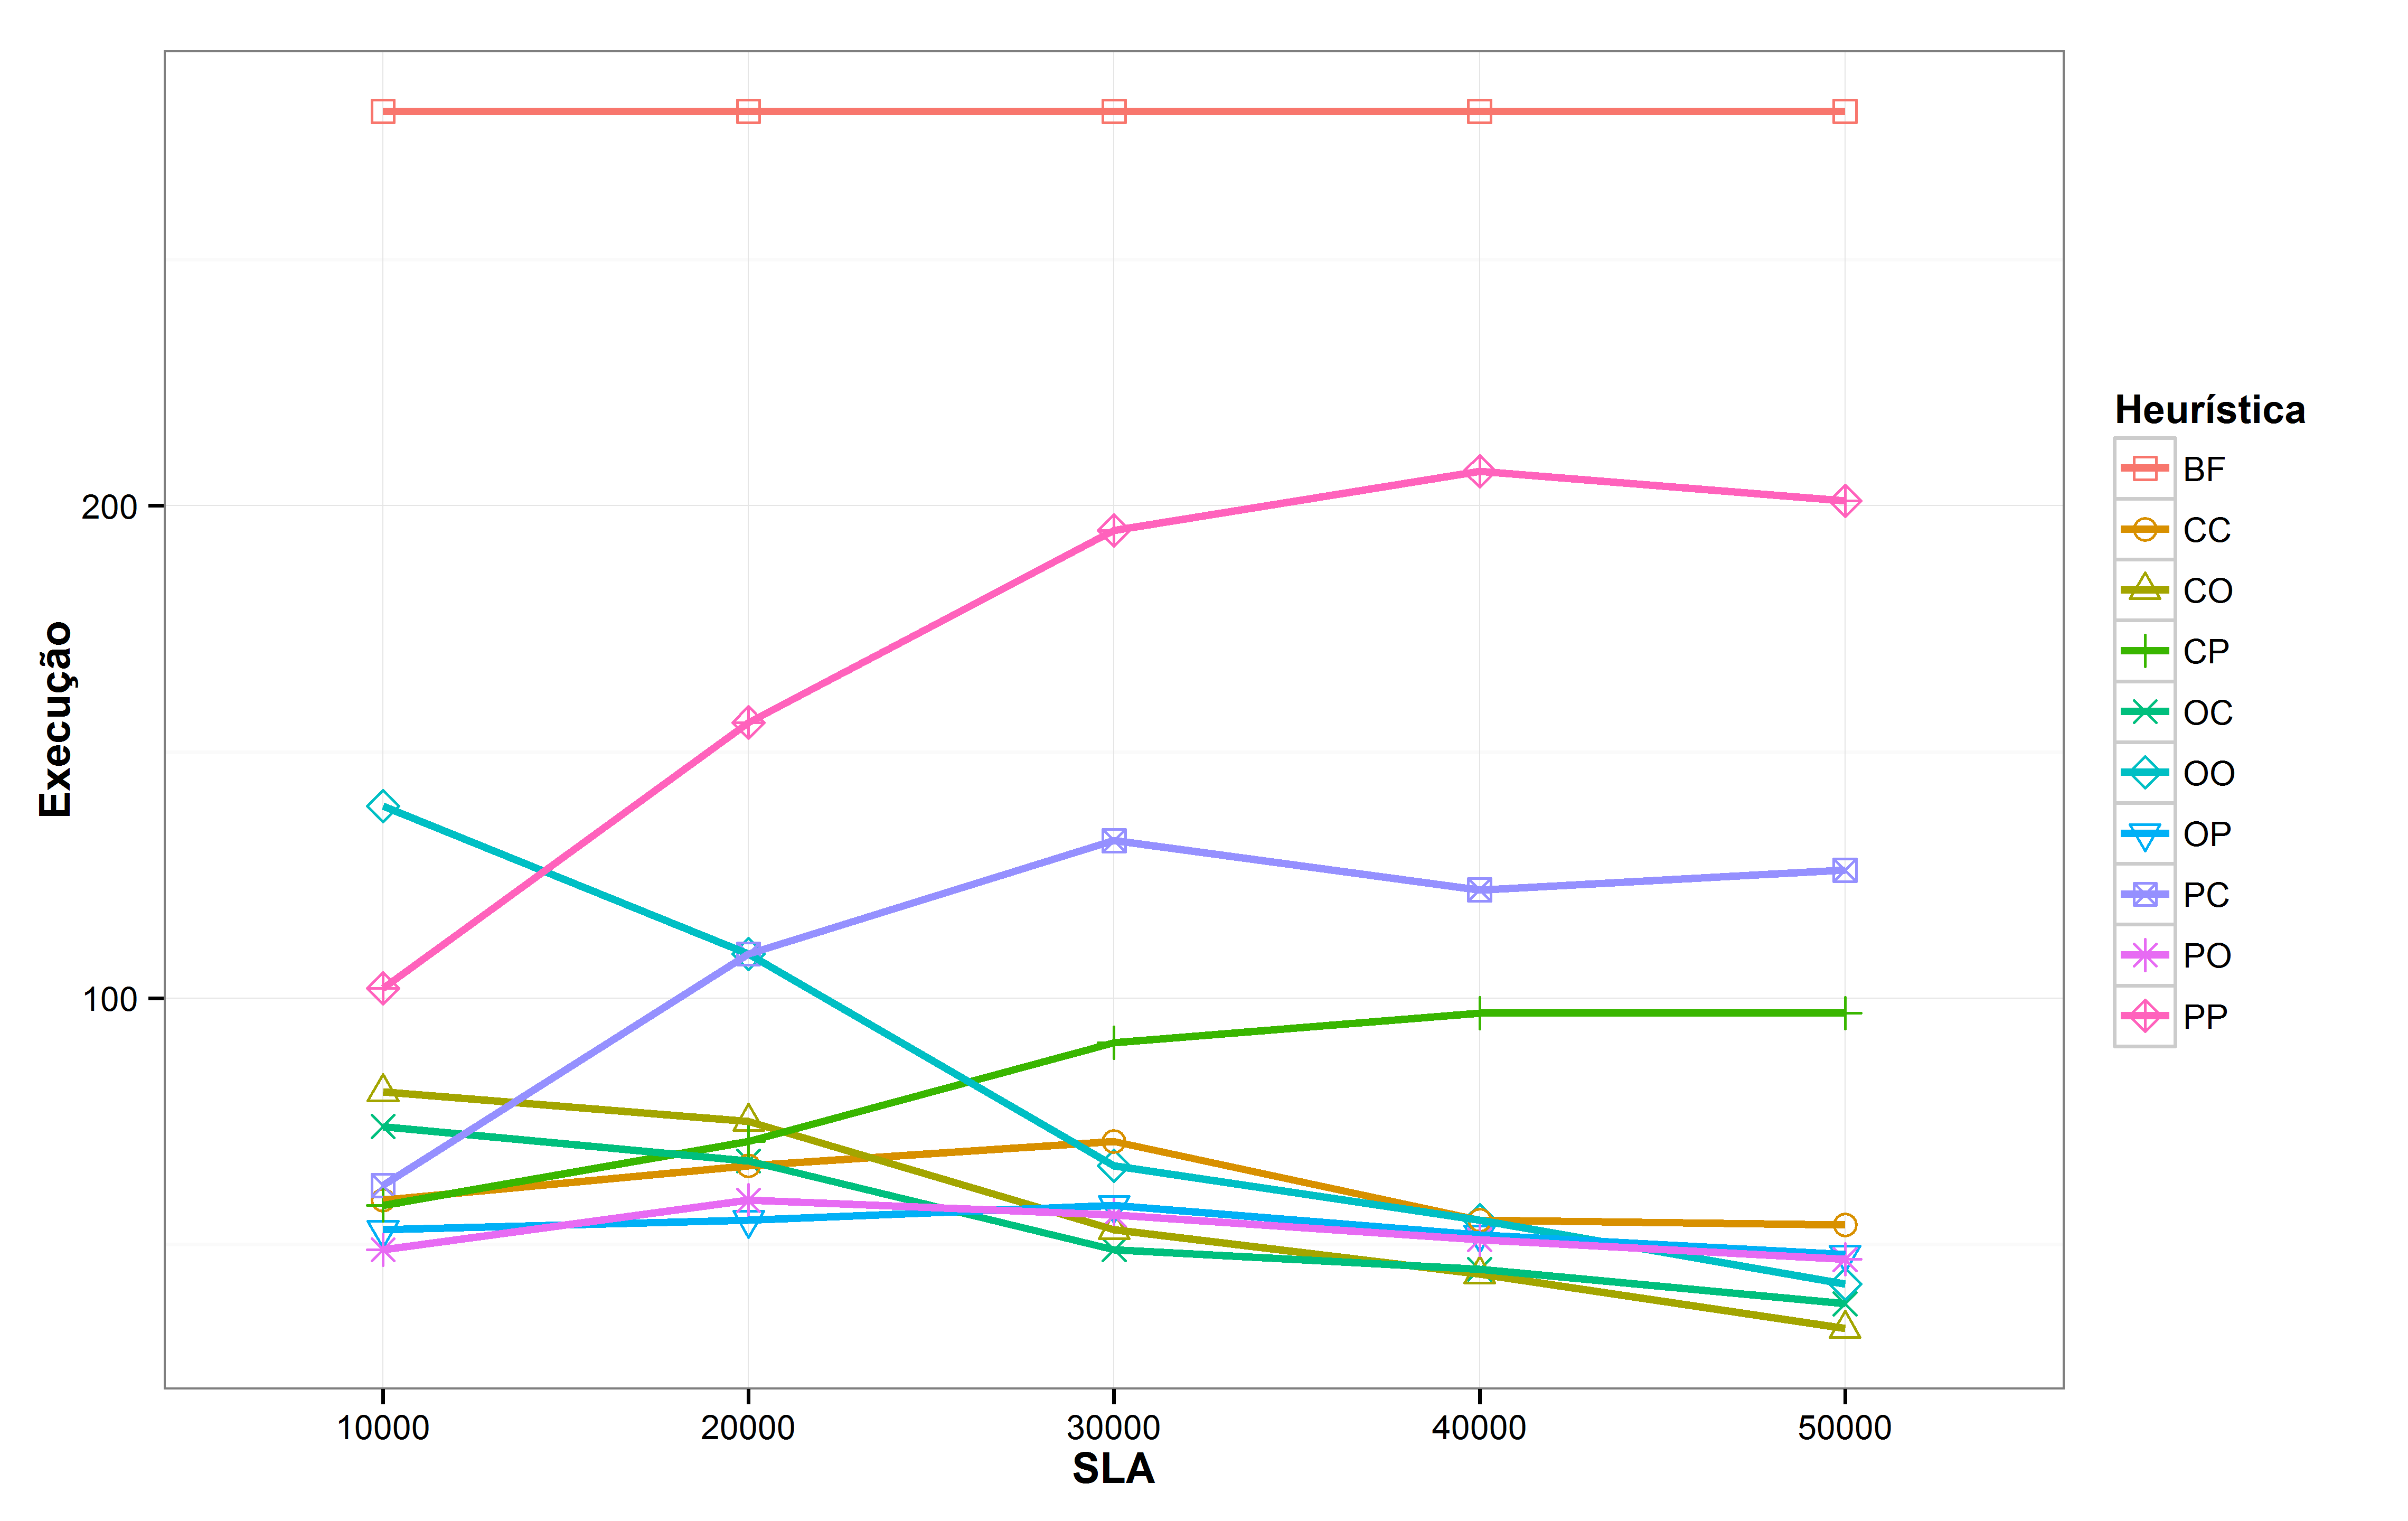
\includegraphics[width=\textwidth]{img/ExecutionCount-Capacity}
      \caption{Grafo por Capacidade}
      \label{fig:eficiencia_custo_capacidade}
    \end{subfigure}
    \begin{subfigure}[b]{0.7\textwidth}
      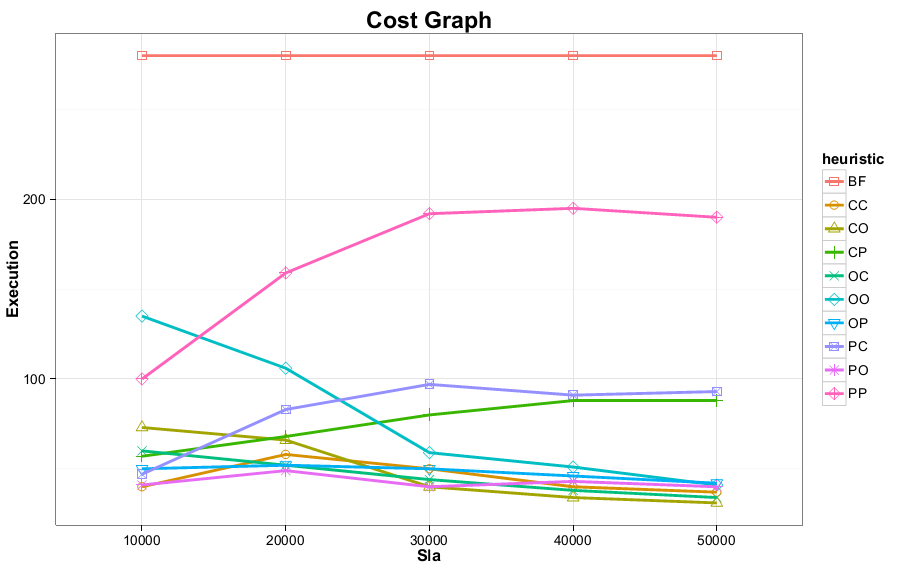
\includegraphics[width=\textwidth]{img/ExecutionCount-Price}
      \caption{Grafo por Preço}
      \label{fig:eficiencia_custo_preco}
    \end{subfigure}
\end{figure}
  
% ----------------------------------------------------------
